% SynthAug-Bench capstone report.
% Structure follows the course's Sample_Report.tex; setup is in File_Setup.tex.
% Compile: pdflatex main, bibtex main, pdflatex main, pdflatex main.

\documentclass{scrartcl}

% Adapted from an original template by Hlyni Arnórssyni, Reykjavik University, Iceland
%
% ------------------------------ SETTINGS
\usepackage{geometry}

\geometry{
	paper=a4paper, % Paper size
	top=2.5cm, % Top margin
	bottom=2.5cm, % Bottom margin
	left=2.5cm, % Left margin
	right=2.4cm, % Right margin
	headheight=0.75cm, % Header height
	footskip=1.5cm, % Space from the bottom margin to the baseline of the footer
	headsep=0.75cm, % Space from the top margin to the baseline of the header
	%showframe, % Uncomment to show how the type block is set on the page
}

\usepackage{blindtext}
%-------------------------------- Character encoding ----------------------------
\usepackage[T1]{fontenc}
\usepackage[utf8]{inputenc}

%----------------------------- Mathematics packages from AMS ---------------

\usepackage{amsmath, amsfonts, amsthm, amssymb}
\usepackage{braket, nicefrac}

% ----------- International System of Units
\usepackage{siunitx}

%------------------------------ Lists / numbers -------------------------
\usepackage{enumitem, multicol}

%------------------------------- Figure insertions --------------
\usepackage{graphicx, float}  % Use option [H] to force the placement of a figure
\usepackage{keystroke}
\usepackage{pgfplots}\usepgfplotslibrary{units}\pgfplotsset{compat=1.16}




%%%%%%%%%%%%%%%%%%%%%%%%%% Hyperlink References %%%%%%%%%%%%%%%%%%%%%%%%%%%
\usepackage{hyperref}

%--------------------% Storage Path for images %-----------------%
\graphicspath{{graphics/}{Graphics/}{./}}
\usepackage{graphicx,epsfig}
\usepackage{booktabs}
\hypersetup{
   colorlinks   = true,
   urlcolor     = blue,
   linkcolor    = blue,
   citecolor    = red,
   setpagesize  = false,
   linktocpage  = true,
}
\graphicspath{ {fig/} }

\renewenvironment{abstract}{
    \centering
    \textbf{Abstract}
    \vspace{0.5cm}
    \par\itshape
    \begin{minipage}{0.7\linewidth}}{\end{minipage}
    \noindent\ignorespaces
}
% ------------------------------------------------------------------------------------------------------------------------

\begin{document}
\begin{titlepage}
	\centering
	
\includegraphics[width=0.6\textwidth]{GW_logo.eps}\par
	\vspace{2cm}
	{\scshape\LARGE Data Science Program \par}
	\vspace{1cm}
	{\scshape\Large Capstone Report - Fall 2026\par}
	\vspace{1.5cm}
	{\huge\bfseries SynthAug-Bench: When Does Diffusion-Based Synthetic Data Augmentation Help?\par}
	\vspace{2cm}
	% Complete the second author's full name.
	{\Large\itshape Mayur Patil,\\ Manoj\\}\par
	\vspace{1.5cm}
	supervised by\par
	Amir Jafari

	\vfill
	\begin{abstract}
	    % Write last, once results exist. Five sentences: (1) what this study shows, (2) why the question
	    % is hard and matters, (3) how it is tested, (4) the evidence, (5) the most important number.
	    % Every claim here must be supported by a result in Section 5.
	    Text-to-image diffusion models can generate unlimited class-conditioned training images, but
	    it is unclear when adding them improves a classifier. This project builds a controlled benchmark
	    that compares pretrained and adapted diffusion augmentation against real-only training and
	    conventional augmentation across data budgets, classifier architectures, and initializations.
	\end{abstract}
	\vfill
\end{titlepage}
\tableofcontents
\newpage
% ------------------------------------------------------------------------------------------------------------------------
\section{Introduction}

% The problem, why it matters, what this project does, and what it found.
% Draw on proposal.md, Sections 1 and 3. End with 2-4 contribution bullets, one or two lines each.

\begin{figure}[htbp]
	\centering
	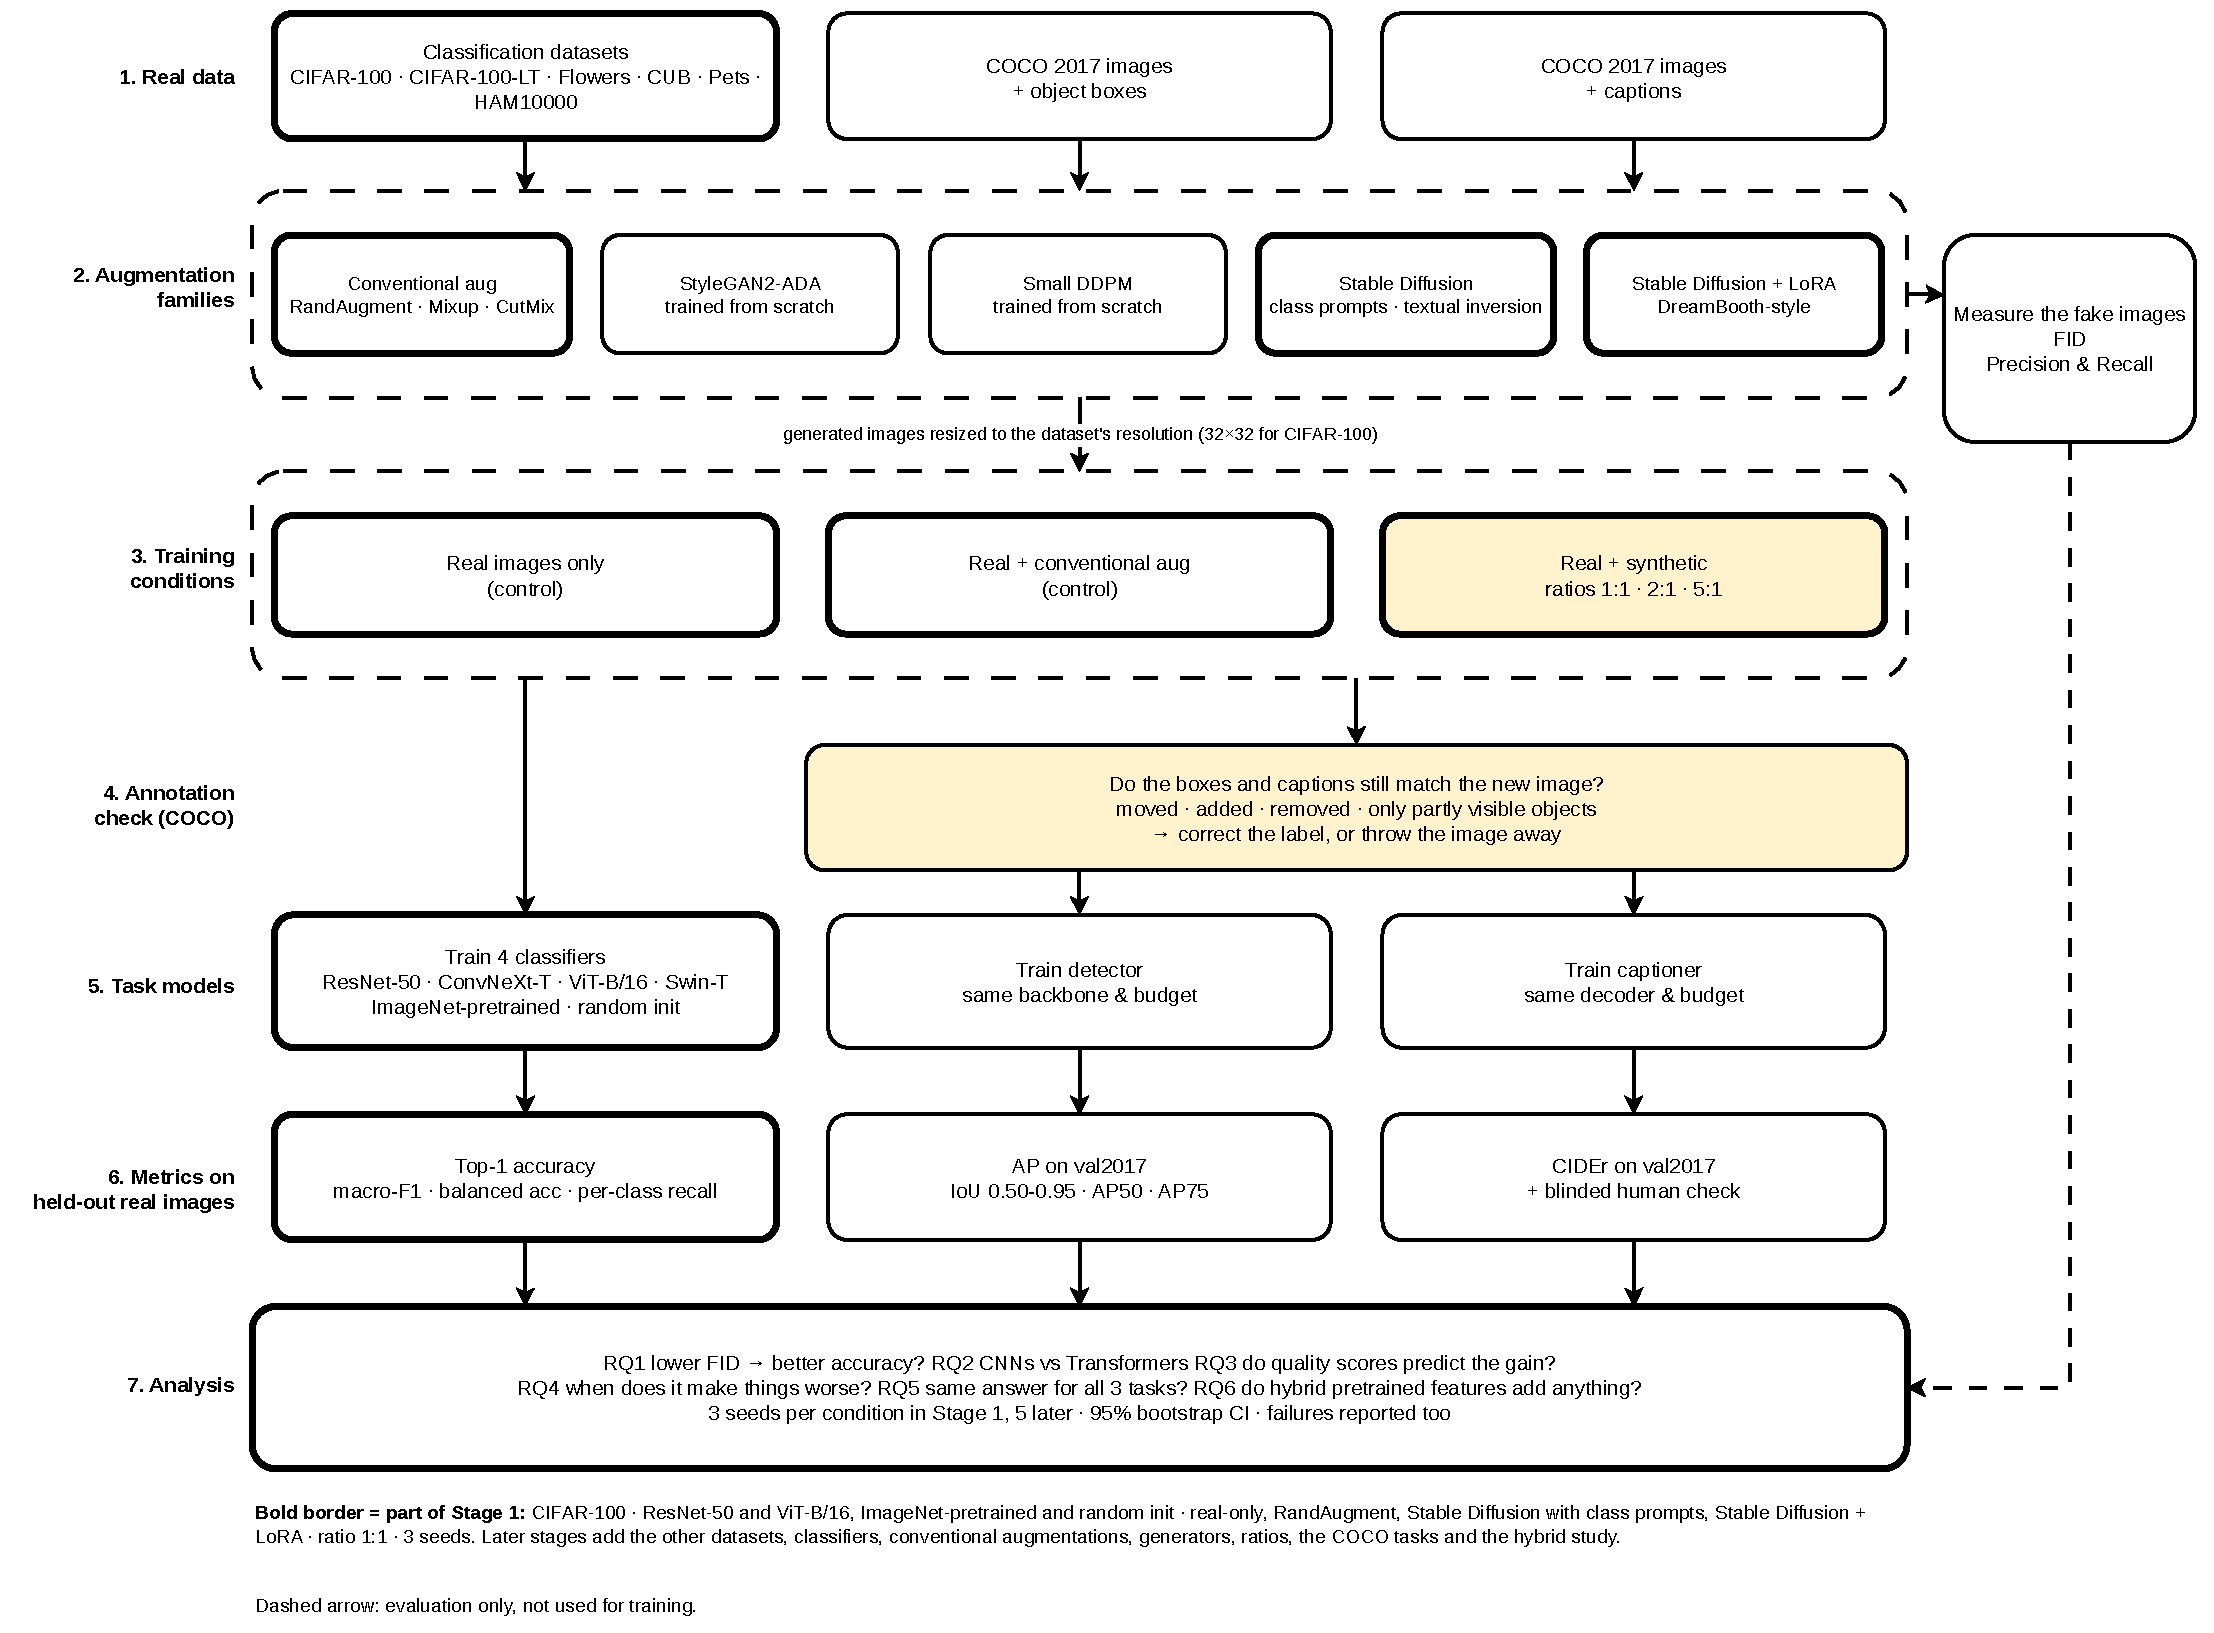
\includegraphics[width=\textwidth]{pipeline-1-architecture.pdf}
	\caption{Overview of SynthAug-Bench. Real images from the classification datasets and MS COCO 2017 feed
	the augmentation families; generated images are resized to the dataset's resolution before training,
	and the boxes and captions of generated COCO images are audited. Task models are scored on held-out
	real images, and the analysis answers the six research questions. Boxes with a bold border are part of
	Stage 1; dashed arrows are used for evaluation only, never for training.}
	\label{fig:overview}
\end{figure}
% Editable source: fig/pipeline.drawio (page 1); SVG export: fig/pipeline-1-architecture.drawio.svg.
% Use one term per concept throughout (e.g. "real-only", "data budget", "generated images").

% ------------------------------------------------------------------------------------------------------------------------
\section{Problem Statement}

% The research questions (proposal.md, RQ1-RQ6) and the challenges: data scarcity, generated images
% that change class-defining details, resolution mismatch between real and generated images,
% seed variation, and compute limits.

% ------------------------------------------------------------------------------------------------------------------------
\section{Related Work}
\label{sec:related}

\subsection{Diffusion models and their adaptation}
A prominent line of research focuses on diffusion models and how to adapt them to new concepts. Ho et al.~\cite{ho2020denoising} introduced models that learn to undo noise step by step, allowing them to create images from pure noise. Rombach et al.~\cite{rombach2022high} made this cheaper by operating in a compressed latent space and adding text control via cross-attention, which forms the basis of Stable Diffusion. Because pretrained models only know what they saw during training, Gal et al.~\cite{gal2023image} proposed textual inversion to teach a frozen model one new ``word'' for a concept using a few images. Ruiz et al.~\cite{ruiz2023dreambooth} developed DreamBooth, which fine-tunes the entire model on a few images using a rare token and an extra loss so it does not forget original classes. Hu et al.~\cite{hu2022lora} introduced LoRA to train small low-rank matrices while freezing the main weights, offering a cheap adaptation method originally for language models but now common for diffusion. In contrast, this study combines LoRA with a DreamBooth-style token, training one specific adapter per data budget using only that budget's real images.

\subsection{Diffusion-based augmentation for classification}
A related approach uses diffusion models to edit existing real images for data augmentation. Trabucco et al.~\cite{trabucco2024effective} use image-to-image translation combined with a learned textual-inversion token for each class. They found that changing the background or pose while keeping the main object helps few-shot learning, even for plants the model never saw during training. Dunlap et al.~\cite{dunlap2023diversify} take this further by captioning real images and using a language model to suggest new domains, like different weather conditions. They edit the images to fit these new domains and filter out poor results, which beats normal augmentation on fine-grained data. In contrast, this study generates entirely new images from scratch instead of editing existing ones, and measures exactly when this helps across increasing data budgets from five examples up to the full set.

\subsection{Synthetic images as training data}
Another line of work trains classifiers on images generated from class names or captions. He et al.~\cite{he2023synthetic} generate images with GLIDE using diverse prompts and filter them with CLIP, finding that synthetic data helps few-shot learning, though this gain shrinks as real data grows. Sariyildiz et al.~\cite{sariyildiz2023fake} train models solely on ``ImageNet clones'' made with Stable Diffusion, showing that prompt variety and lower guidance scale help these models transfer well to other datasets. Azizi et al.~\cite{azizi2023synthetic} fine-tune Imagen on all of ImageNet and show that adding the resulting synthetic images back into the real dataset improves accuracy. Lastly, Tian et al.~\cite{tian2023stablerep} learn representations by treating Stable Diffusion images with the same caption as positive pairs, achieving results comparable to training on real images. In contrast, this study adds synthetic images to scarce real data at a strict one-to-one ratio, restricts the diffusion adapter to only see its specific data budget, and compares the impact on both pretrained and from-scratch classifiers.

\subsection{Conventional augmentation and generators trained from scratch}
Beyond diffusion, other research relies on conventional data augmentation and generative models trained entirely from scratch. Cubuk et al.~\cite{cubuk2020randaugment} introduced RandAugment, which applies random standard transforms at one shared strength. It avoids an expensive policy search and is the conventional-augmentation baseline in this study. Karras et al.~\cite{karras2020training} developed StyleGAN2-ADA to train a GAN on just a few thousand images by augmenting what the discriminator sees, which prevents overfitting. GANs trained this way know only their training set, whereas Stable Diffusion carries knowledge from billions of outside images; GANs are planned for a later stage.

\subsection{Measuring generated-image quality}
A separate focus is measuring the quality of generated images. Heusel et al.~\cite{heusel2017gans} created the Fréchet Inception Distance (FID), which measures the distance between real and fake images using Inception features, where a lower score means higher similarity. Kynkäänniemi et al.~\cite{kynkaanniemi2019improved} improved on this by using k-nearest-neighbor regions to separate an image's realism (precision) from its variety (recall). Parmar et al.~\cite{parmar2022aliased} introduced Clean-FID to fix how FID scores inconsistently change with image resizing and compression. This study uses Clean-FID features, compares sets of equal size and reports a real-versus-real floor, so it can ask whether better FID leads to better accuracy.

\subsection{Beyond classification}
Recent work has also expanded generative data augmentation beyond simple image classification tasks. For example, Fang et al.~\cite{fang2024data} use controllable diffusion models to generate new objects directly inside bounding boxes. This creates labeled synthetic data for training object detection systems. Similarly, Xiao et al.~\cite{xiao2023multimodal} generate diverse images from existing captions to produce more training data for image captioning models. While both approaches help in low-data settings, this study currently focuses strictly on classification, leaving detection and captioning on datasets like COCO for later stages.

\subsection{How this study differs}
In summary, this study differs from prior work through a highly controlled experimental design. It evaluates performance using the exact same protocol across five specific data budgets. The tests span both CNN and Transformer architectures, comparing classifiers trained from scratch against pretrained ones. This study specifically contrasts plain Stable Diffusion with per-budget LoRA adapters, ensuring training steps are matched so any accuracy gain is not simply from training longer. Furthermore, generated images are reduced to 32×32, the size of the real images, and this study compares the synthetic data with RandAugment and with the two combined. Finally, this study uses paired seeds to provide an explicit per-seed verdict on exactly when generative augmentation succeeds.

% ------------------------------------------------------------------------------------------------------------------------
\section{Solution and Methodology}

\subsection{Dataset and splits}
% CIFAR-100 \cite{krizhevsky2009learning}: 50 validation images per class (split seed 42), nested
% training budgets of 5, 10, 20, 50 images per class and the full 45,000; official test set held out.
% See src/docs/data-splits.md.

\subsection{Classifiers and training protocol}
% ResNet-50 \cite{he2016deep} and ViT-B/16 \cite{dosovitskiy2021image}; ImageNet-pretrained and randomly
% initialized arms; recipe, step budgets and checkpoint rule from the pilot. See src/docs/training.md.

\subsection{Augmentation conditions}
% Real-only, RandAugment, pretrained Stable Diffusion, LoRA-adapted Stable Diffusion; generated images
% resized to 32x32 before the shared preprocessing.

Stage 1 compares five training conditions, each defined as one change to the real-only control. \textit{Real-only} trains on the real images of the budget without augmentation. \textit{RandAugment} applies two RandAugment operations at magnitude 9 to every training image. \textit{Pretrained Stable Diffusion} adds generated images to the real-only training set, one generated image per real image (synthetic:real 1:1): for a budget of $k$ images per class, the first $k$ generated images of each class are added, so the generated sets are nested across budgets in the same way as the real ones. \textit{Pretrained Stable Diffusion with RandAugment} uses the same pool and applies RandAugment to every image, so that a gain from generated images can be separated from the gain of augmentation in general. \textit{LoRA-adapted Stable Diffusion} replaces the pool with images from an adapter fitted only on the real images of the same budget, so each budget has its own generated set.

Generated images are resized to $32\times32$ before training and then follow exactly the same preprocessing as the real images, so a classifier cannot separate the two by resolution or sharpness. Batches sample the combined pool uniformly, so about half of each batch is generated. Because the step budget stays the same as for real-only training, each image is seen about half as often as in the real-only run. Every run records a fingerprint of the generated pool, the synthetic:real ratio and the number of generated images it used.

\subsection{Evaluation}
% Top-1 accuracy, macro-F1, per-class recall; paired changes per seed; bootstrap intervals.

\begin{figure}[htbp]
	\centering
	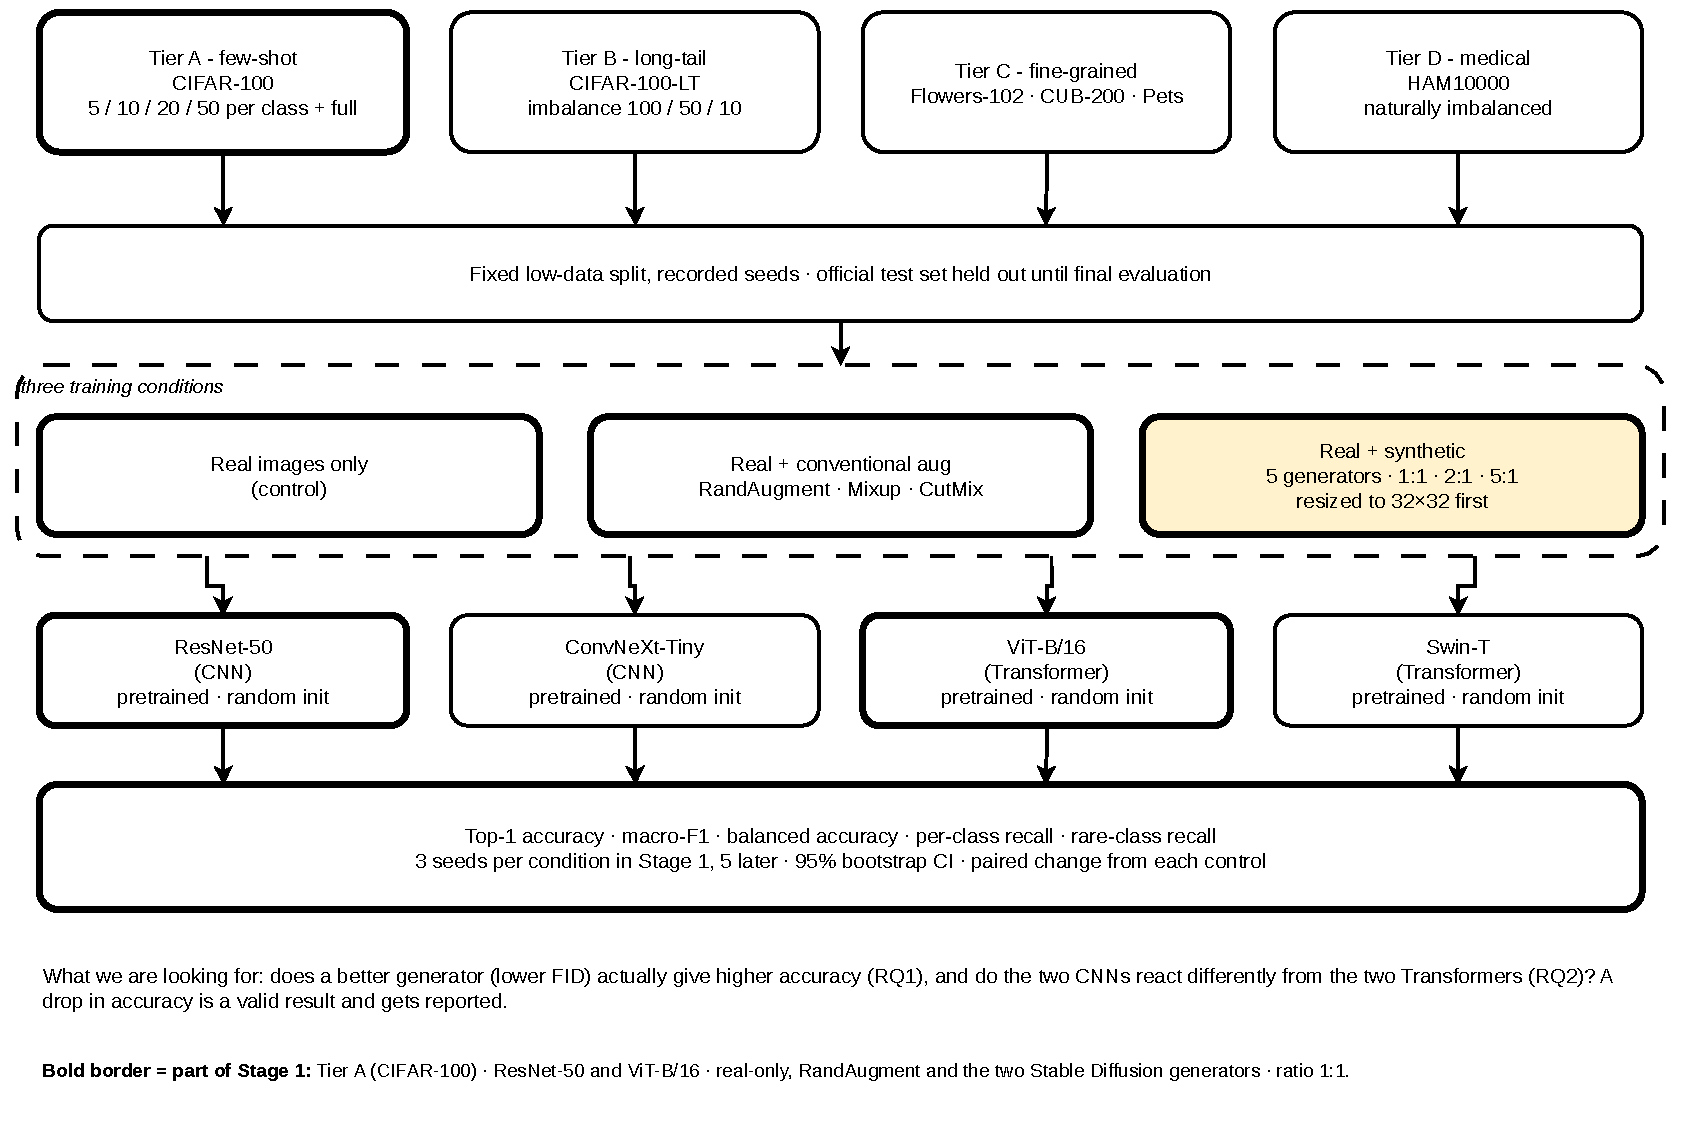
\includegraphics[width=\textwidth]{pipeline-2-classification.pdf}
	\caption{Classification study design. Each data tier is split once with recorded seeds, and the official
	test set is held out until the final evaluation. Every classifier, pretrained and randomly initialized,
	is trained under three conditions: real images only, real images with conventional augmentation, and
	real images with generated images, which are resized to the dataset's resolution first. Boxes with a
	bold border are part of Stage 1.}
	\label{fig:classification-design}
\end{figure}
% Editable source: fig/pipeline.drawio (page 2); SVG export: fig/pipeline-2-classification.drawio.svg.

% ------------------------------------------------------------------------------------------------------------------------
\section{Results and Discussion}

% Before each experiment, state the claim it tests. Report mean and standard deviation over seeds
% (say which), the number of runs, and the paired changes. Tables use booktabs with consistent
% decimals; figures are vector (SVG or PDF) with self-contained captions and colorblind-safe colors.

\subsection{Experimentation protocol}
\label{sec:protocol}
% Hardware (NVIDIA A10G, 24 GB), software versions, total GPU hours, number of runs, seeds,
% and how the learning rates and step budgets were chosen (pilot, seed 100, validation only).

All runs used NVIDIA A10G GPUs (24\,GB). The pilots and the real-only and RandAugment runs used Python 3.12.14, PyTorch 2.12.1 (CUDA 12.6), Torchvision 0.27.1 and NumPy 2.5.2, the versions pinned in the environment file. The synthetic-data runs were trained on a second A10G instance with Python 3.13.14, PyTorch 2.13.0 (CUDA 13.0), Torchvision 0.28.0 and NumPy 2.4.4. The CIFAR-100 split is fixed by a manifest with seed 42: 50 images per class (5,000 in total) are held out from the training pool for validation, and the 5, 10, 20 and 50 images-per-class budgets are nested subsets of the remaining 45,000 images, which form the full budget. The official 10,000-image test set is not used before the protocol is final.

ResNet-50 and ViT-B/16 are trained with all layers updated, either from ImageNet weights (torchvision \texttt{IMAGENET1K\_V2} and \texttt{IMAGENET1K\_V1}) or from random initialization. Images stay at $32\times32$ until they are upsampled to $224\times224$ on the GPU and normalized with the ImageNet statistics. Every run uses batch size 128, linear warmup over the first 5\% of steps followed by cosine decay to zero, label smoothing 0.1, gradient-norm clipping at 1.0 and bf16 mixed precision. The real-only condition applies no augmentation; RandAugment applies two operations at magnitude 9 to the $32\times32$ image.

The learning rates and optimizer-step budgets were chosen in pilot runs with seed 100, on validation accuracy only (38 runs, 21.2 GPU hours). The pretrained arm uses AdamW with weight decay 0.05 and learning rate $3\times10^{-4}$ for ResNet-50 and $5\times10^{-5}$ for ViT-B/16, for 600, 800, 1,000, 1,500 and 6,000 steps at the five budgets. The random-initialization arm uses SGD with momentum 0.9, weight decay $5\times10^{-4}$ and learning rate 1.0 for ResNet-50, and AdamW with weight decay 0.05 and learning rate $3\times10^{-4}$ for ViT-B/16, for 2,000, 3,000, 4,000, 8,000 and 50,000 steps. Within an arm, every condition of a given budget uses the same recipe and step budget.

Each run is validated 20 times at equal step intervals and keeps the checkpoint with the highest validation accuracy, breaking ties by the lower validation loss and then the earlier step. Runs are seeded with training seeds 0, 1 and 2, and the batch order and per-sample augmentation are fixed functions of the seed and the step. The 120 baseline runs took 88.4 GPU hours (12.5 for the pretrained arm, 75.9 for the random-initialization arm), with peak GPU memory of 5.7\,GiB for ResNet-50 and 9.7\,GiB for ViT-B/16.

We compare conditions by the paired change for each training seed: the treatment score minus the control score of the same seed, in percentage points. A change counts as a gain or a loss only when all three seeds agree in sign; otherwise it is reported as inconclusive. Tables give the mean and sample standard deviation over the three seeds.

\subsection{Baselines}
% Real-only and RandAugment results per model and data budget.

Table~\ref{tab:stage1-pretrained-accuracy} and Figure~\ref{fig:stage1-pretrained-accuracy} show the ImageNet-pretrained baselines on the validation split.

\begin{table}[H]
\centering
\caption{Stage 1 baselines, pretrained initialization: validation top-1 accuracy (\%), mean $\pm$ sample SD over 3 seeds. The change is RandAugment minus real-only per seed (percentage points); it is a gain or a loss only when every seed agrees in sign.}
\label{tab:stage1-pretrained-accuracy}
\begin{tabular}{llrrrl}
\toprule
Model & Images/class & Real-only & RandAugment & Change & Verdict \\
\midrule
ResNet-50 & 5 & 35.17 $\pm$ 0.86 & 43.03 $\pm$ 0.99 & +7.85 $\pm$ 1.72 & gain \\
ResNet-50 & 10 & 49.51 $\pm$ 0.96 & 53.49 $\pm$ 0.45 & +3.99 $\pm$ 0.65 & gain \\
ResNet-50 & 20 & 59.48 $\pm$ 0.33 & 63.11 $\pm$ 0.52 & +3.63 $\pm$ 0.54 & gain \\
ResNet-50 & 50 & 71.36 $\pm$ 0.39 & 72.19 $\pm$ 0.29 & +0.83 $\pm$ 0.12 & gain \\
ResNet-50 & full & 84.17 $\pm$ 0.19 & 85.17 $\pm$ 0.10 & +1.00 $\pm$ 0.11 & gain \\
\midrule
ViT-B/16 & 5 & 46.93 $\pm$ 1.61 & 57.03 $\pm$ 2.11 & +10.09 $\pm$ 0.59 & gain \\
ViT-B/16 & 10 & 61.08 $\pm$ 1.40 & 69.25 $\pm$ 1.49 & +8.17 $\pm$ 1.03 & gain \\
ViT-B/16 & 20 & 72.05 $\pm$ 1.08 & 76.21 $\pm$ 0.52 & +4.15 $\pm$ 0.56 & gain \\
ViT-B/16 & 50 & 80.29 $\pm$ 0.09 & 82.03 $\pm$ 0.52 & +1.74 $\pm$ 0.58 & gain \\
ViT-B/16 & full & 88.64 $\pm$ 0.02 & 89.89 $\pm$ 0.28 & +1.25 $\pm$ 0.29 & gain \\
\bottomrule
\end{tabular}
\end{table}

% Generated by src/component/analyze_results.py --table; CSV copies are in tables/.

\begin{figure}[H]
	\centering
	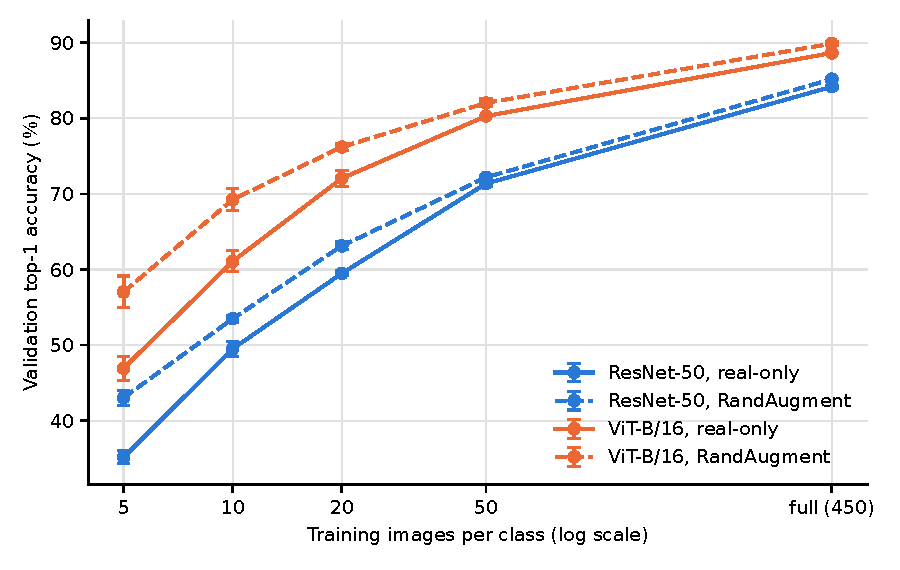
\includegraphics[width=0.8\textwidth]{stage1_pretrained_accuracy.pdf}
	\caption{Validation top-1 accuracy of the ImageNet-pretrained baselines against training images per class (log scale). Points are means over seeds 0, 1 and 2 with $\pm 1$ standard deviation; color marks the classifier and line style the condition.}
	\label{fig:stage1-pretrained-accuracy}
\end{figure}
% Generated by src/component/analyze_results.py --figure; the SVG copy is in fig/.

Table~\ref{tab:stage1-scratch-accuracy} and Figure~\ref{fig:stage1-scratch-accuracy} show the same comparison with randomly initialized classifiers.

\begin{table}[H]
\centering
\caption{Stage 1 baselines, scratch initialization: validation top-1 accuracy (\%), mean $\pm$ sample SD over 3 seeds. The change is RandAugment minus real-only per seed (percentage points); it is a gain or a loss only when every seed agrees in sign.}
\label{tab:stage1-scratch-accuracy}
\begin{tabular}{llrrrl}
\toprule
Model & Images/class & Real-only & RandAugment & Change & Verdict \\
\midrule
ResNet-50 & 5 & 8.85 $\pm$ 0.36 & 14.88 $\pm$ 0.58 & +6.03 $\pm$ 0.81 & gain \\
ResNet-50 & 10 & 13.30 $\pm$ 0.69 & 22.65 $\pm$ 0.78 & +9.35 $\pm$ 0.78 & gain \\
ResNet-50 & 20 & 19.19 $\pm$ 0.29 & 29.74 $\pm$ 2.50 & +10.55 $\pm$ 2.78 & gain \\
ResNet-50 & 50 & 29.71 $\pm$ 1.30 & 39.33 $\pm$ 3.40 & +9.61 $\pm$ 4.70 & gain \\
ResNet-50 & full & 54.98 $\pm$ 0.99 & 65.27 $\pm$ 1.28 & +10.29 $\pm$ 1.63 & gain \\
\midrule
ViT-B/16 & 5 & 7.43 $\pm$ 0.27 & 9.96 $\pm$ 0.07 & +2.53 $\pm$ 0.32 & gain \\
ViT-B/16 & 10 & 10.03 $\pm$ 0.31 & 13.39 $\pm$ 0.01 & +3.37 $\pm$ 0.31 & gain \\
ViT-B/16 & 20 & 13.55 $\pm$ 0.28 & 18.12 $\pm$ 0.50 & +4.57 $\pm$ 0.69 & gain \\
ViT-B/16 & 50 & 19.51 $\pm$ 0.46 & 27.69 $\pm$ 0.21 & +8.17 $\pm$ 0.34 & gain \\
ViT-B/16 & full & 44.18 $\pm$ 0.47 & 59.15 $\pm$ 0.31 & +14.97 $\pm$ 0.71 & gain \\
\bottomrule
\end{tabular}
\end{table}


\begin{figure}[H]
	\centering
	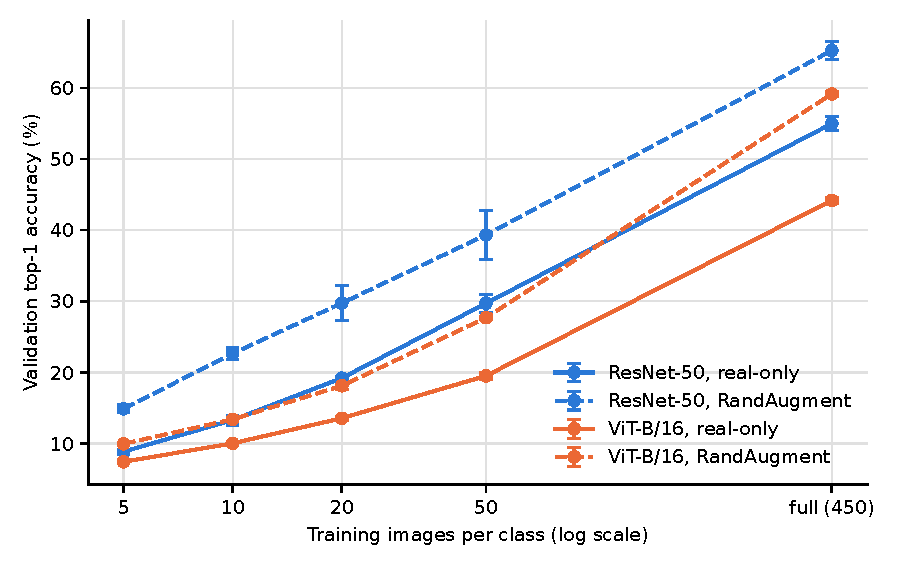
\includegraphics[width=0.8\textwidth]{stage1_scratch_accuracy.pdf}
	\caption{Validation top-1 accuracy of the randomly initialized baselines against training images per class (log scale). Points are means over seeds 0, 1 and 2 with $\pm 1$ standard deviation; color marks the classifier and line style the condition.}
	\label{fig:stage1-scratch-accuracy}
\end{figure}

\subsection{Synthetic-data augmentation}
% Pretrained and adapted diffusion conditions, as paired changes from the matched baselines.

This section tests whether adding generated images to the real training images improves validation accuracy, compared with real-only training and with RandAugment, and whether the answer depends on the data budget and on the classifier's initialization. Every synthetic run uses the recipe and step budget of the real-only run of the same budget and pairs with it by training seed.

\textbf{Generated-image quality.} Figure~\ref{fig:sd-samples} shows class-prompt samples. Against an equal number of real training images, the class-prompt pool reaches an FID of 34.2 at 50 images per class (5,000 images) and 24.7 at the full budget (45,000 images); two disjoint sets of 5,000 real images give 11.9. The LoRA pools have lower FID than the class-prompt pool from 10 images per class upward (30.2 against 34.2 at 50 per class) and higher recall (0.37 against 0.29), at lower precision (0.65 against 0.72). All scores are in \texttt{tables/generator\_quality.csv}.

\begin{figure}[H]
	\centering
	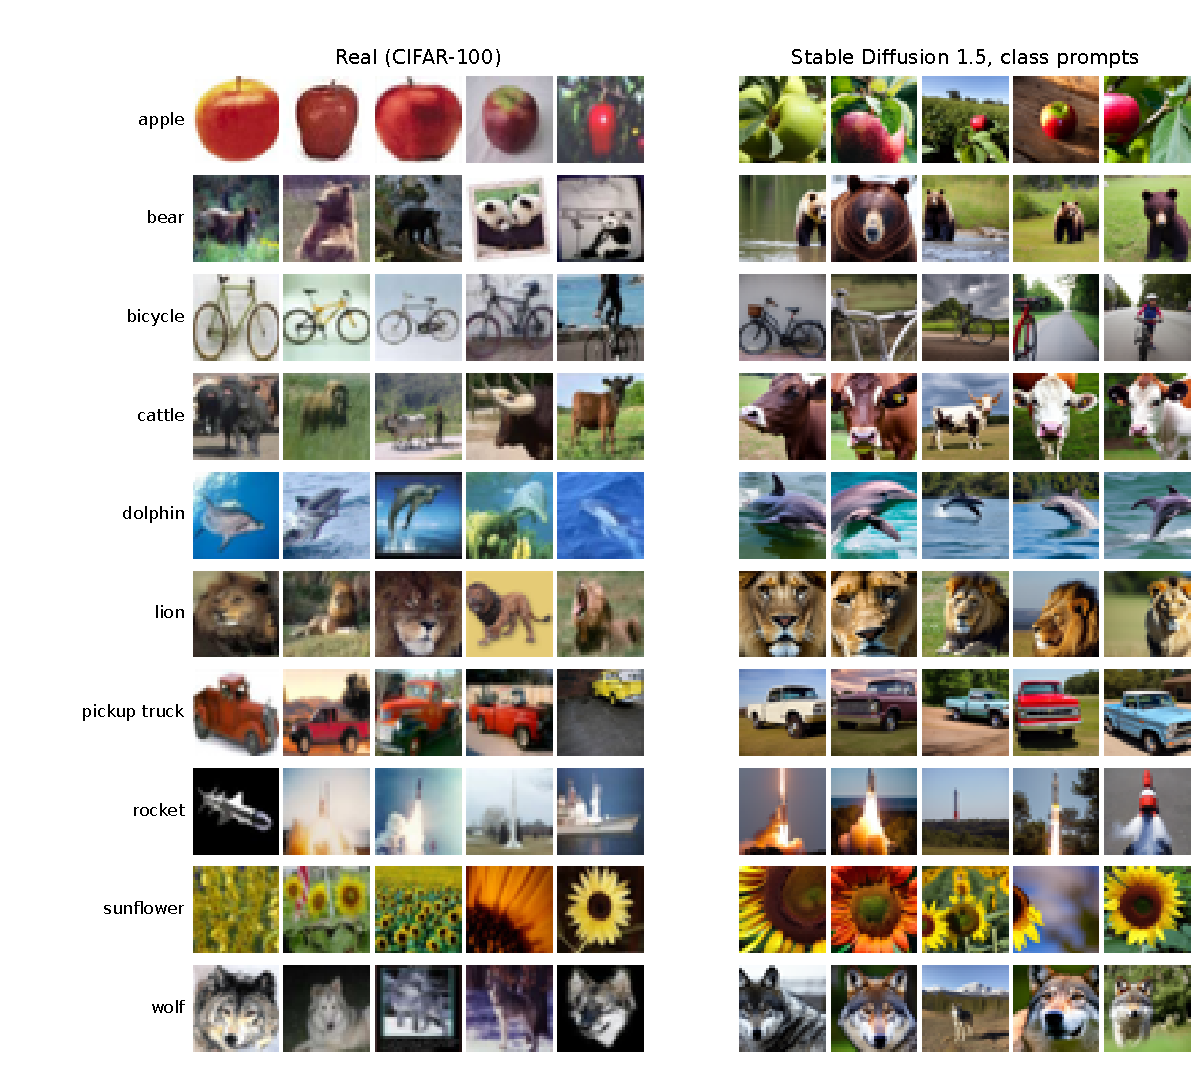
\includegraphics[width=0.8\textwidth]{sd15_prompt_samples.pdf}
	\caption{Samples of the class-prompt pool (pretrained Stable Diffusion 1.5, 32$\times$32 as used for training).}
	\label{fig:sd-samples}
\end{figure}

\textbf{ImageNet-pretrained classifiers.} Adding class-prompt images helps most when real data is scarce (Table~\ref{tab:stage1-pretrained-accuracy-sd_prompt}): at 5 images per class, accuracy rises by 11.6 points for ResNet-50 and 14.4 points for ViT-B/16, the gain shrinks with the budget, and at the full budget the change is inconclusive for both. Against RandAugment (Table~\ref{tab:stage1-pretrained-accuracy-vs-randaugment}), the generated images alone remain ahead at small budgets (+3.8 and +4.3 points at 5 per class) but fall behind at the full budget. Combined with RandAugment, they add to the augmentation: SD with RandAugment exceeds RandAugment alone by 9.6 points (ResNet-50) and 11.2 points (ViT-B/16) at 5 images per class and still gains at 50 per class, with inconclusive changes at the full budget. LoRA adaptation, despite its lower FID, helps less than the class prompts at every budget: against RandAugment it gains up to 20 images per class for ResNet-50 but only at 5 per class for ViT-B/16, and loses for ViT-B/16 from 10 images per class upward.

\begin{table}[H]
\centering
\caption{Stage 1, SD class prompts against real-only, pretrained initialization: validation top-1 accuracy (\%), mean $\pm$ sample SD over 3 seeds. The change is SD class prompts minus real-only per seed (percentage points); it is a gain or a loss only when every seed agrees in sign.}
\label{tab:stage1-pretrained-accuracy-sd_prompt}
\begin{tabular}{llrrrl}
\toprule
Model & Images/class & Real-only & SD class prompts & Change & Verdict \\
\midrule
ResNet-50 & 5 & 35.17 $\pm$ 0.86 & 46.78 $\pm$ 0.19 & +11.61 $\pm$ 0.98 & gain \\
ResNet-50 & 10 & 49.51 $\pm$ 0.96 & 57.03 $\pm$ 0.95 & +7.52 $\pm$ 1.64 & gain \\
ResNet-50 & 20 & 59.48 $\pm$ 0.33 & 65.49 $\pm$ 0.22 & +6.01 $\pm$ 0.37 & gain \\
ResNet-50 & 50 & 71.36 $\pm$ 0.39 & 73.50 $\pm$ 0.23 & +2.14 $\pm$ 0.24 & gain \\
ResNet-50 & full & 84.17 $\pm$ 0.19 & 84.40 $\pm$ 0.28 & +0.23 $\pm$ 0.37 & inconclusive \\
\midrule
ViT-B/16 & 5 & 46.93 $\pm$ 1.61 & 61.35 $\pm$ 2.14 & +14.42 $\pm$ 0.54 & gain \\
ViT-B/16 & 10 & 61.08 $\pm$ 1.40 & 70.76 $\pm$ 1.22 & +9.68 $\pm$ 0.61 & gain \\
ViT-B/16 & 20 & 72.05 $\pm$ 1.08 & 75.99 $\pm$ 0.96 & +3.94 $\pm$ 0.19 & gain \\
ViT-B/16 & 50 & 80.29 $\pm$ 0.09 & 81.09 $\pm$ 0.62 & +0.80 $\pm$ 0.71 & gain \\
ViT-B/16 & full & 88.64 $\pm$ 0.02 & 88.64 $\pm$ 0.26 & +0.00 $\pm$ 0.28 & inconclusive \\
\bottomrule
\end{tabular}
\end{table}


\begin{table}[H]
\centering
\caption{Stage 1 synthetic conditions against RandAugment, pretrained initialization: change in validation top-1 accuracy (percentage points), paired by training seed, mean $\pm$ sample SD over 3 seeds. SD: pretrained Stable Diffusion with class prompts; LoRA: LoRA-adapted Stable Diffusion; RA: RandAugment. $\uparrow$ gain and $\downarrow$ loss when every seed agrees in sign, $\sim$ inconclusive otherwise.}
\label{tab:stage1-pretrained-accuracy-vs-randaugment}
\begin{tabular}{llrrr}
\toprule
Model & Images/class & SD$-$RA & LoRA$-$RA & SD+RA$-$RA \\
\midrule
ResNet-50 & 5 & +3.75 $\pm$ 1.05 $\uparrow$ & +2.17 $\pm$ 1.35 $\uparrow$ & +9.58 $\pm$ 0.63 $\uparrow$ \\
ResNet-50 & 10 & +3.53 $\pm$ 1.37 $\uparrow$ & +1.95 $\pm$ 0.68 $\uparrow$ & +6.49 $\pm$ 0.39 $\uparrow$ \\
ResNet-50 & 20 & +2.38 $\pm$ 0.73 $\uparrow$ & +1.53 $\pm$ 0.98 $\uparrow$ & +3.55 $\pm$ 0.33 $\uparrow$ \\
ResNet-50 & 50 & +1.31 $\pm$ 0.22 $\uparrow$ & +0.11 $\pm$ 0.87 $\sim$ & +2.17 $\pm$ 0.62 $\uparrow$ \\
ResNet-50 & full & -0.77 $\pm$ 0.34 $\downarrow$ & -1.09 $\pm$ 0.48 $\downarrow$ & +0.23 $\pm$ 0.32 $\sim$ \\
\midrule
ViT-B/16 & 5 & +4.33 $\pm$ 0.22 $\uparrow$ & +1.55 $\pm$ 1.22 $\uparrow$ & +11.17 $\pm$ 0.56 $\uparrow$ \\
ViT-B/16 & 10 & +1.51 $\pm$ 0.46 $\uparrow$ & -1.02 $\pm$ 0.49 $\downarrow$ & +4.96 $\pm$ 0.91 $\uparrow$ \\
ViT-B/16 & 20 & -0.21 $\pm$ 0.46 $\sim$ & -1.67 $\pm$ 0.23 $\downarrow$ & +1.83 $\pm$ 0.16 $\uparrow$ \\
ViT-B/16 & 50 & -0.94 $\pm$ 0.38 $\downarrow$ & -1.78 $\pm$ 0.19 $\downarrow$ & +0.57 $\pm$ 0.02 $\uparrow$ \\
ViT-B/16 & full & -1.25 $\pm$ 0.07 $\downarrow$ & -1.77 $\pm$ 0.29 $\downarrow$ & -0.43 $\pm$ 0.59 $\sim$ \\
\bottomrule
\end{tabular}
\end{table}


\textbf{Randomly initialized classifiers.} Without pretraining, class-prompt images still improve over real-only training at every budget, by 1.9 to 8.2 points for ResNet-50 and 1.9 to 4.0 points for ViT-B/16 (\texttt{tables/stage1\_scratch\_accuracy\_sd\_prompt.tex}), but both synthetic conditions fall behind RandAugment at almost every budget (Table~\ref{tab:stage1-scratch-accuracy-vs-randaugment}), by up to 11.0 points for ViT-B/16 at the full budget. The combined SD and RandAugment runs for this arm are still to be trained.

\begin{table}[H]
\centering
\caption{Stage 1 synthetic conditions against RandAugment, scratch initialization: change in validation top-1 accuracy (percentage points), paired by training seed, mean $\pm$ sample SD over 3 seeds. SD: pretrained Stable Diffusion with class prompts; LoRA: LoRA-adapted Stable Diffusion; RA: RandAugment. $\uparrow$ gain and $\downarrow$ loss when every seed agrees in sign, $\sim$ inconclusive otherwise.}
\label{tab:stage1-scratch-accuracy-vs-randaugment}
\begin{tabular}{llrrr}
\toprule
Model & Images/class & SD$-$RA & LoRA$-$RA & SD+RA$-$RA \\
\midrule
ResNet-50 & 5 & -4.11 $\pm$ 1.03 $\downarrow$ & -4.79 $\pm$ 0.44 $\downarrow$ & -- \\
ResNet-50 & 10 & -7.30 $\pm$ 0.65 $\downarrow$ & -7.43 $\pm$ 1.04 $\downarrow$ & -- \\
ResNet-50 & 20 & -5.11 $\pm$ 1.06 $\downarrow$ & -4.57 $\pm$ 2.35 $\downarrow$ & -- \\
ResNet-50 & 50 & -1.39 $\pm$ 2.97 $\sim$ & -2.43 $\pm$ 3.74 $\sim$ & -- \\
ResNet-50 & full & -5.42 $\pm$ 2.30 $\downarrow$ & -3.03 $\pm$ 1.90 $\downarrow$ & -- \\
\midrule
ViT-B/16 & 5 & -0.67 $\pm$ 0.13 $\downarrow$ & -1.06 $\pm$ 0.14 $\downarrow$ & -- \\
ViT-B/16 & 10 & -1.39 $\pm$ 0.63 $\downarrow$ & -1.46 $\pm$ 0.40 $\downarrow$ & -- \\
ViT-B/16 & 20 & -1.97 $\pm$ 0.27 $\downarrow$ & -2.69 $\pm$ 1.19 $\downarrow$ & -- \\
ViT-B/16 & 50 & -4.87 $\pm$ 0.43 $\downarrow$ & -5.36 $\pm$ 0.49 $\downarrow$ & -- \\
ViT-B/16 & full & -11.02 $\pm$ 0.70 $\downarrow$ & -8.89 $\pm$ 0.75 $\downarrow$ & -- \\
\bottomrule
\end{tabular}
\end{table}


\begin{figure}[H]
	\centering
	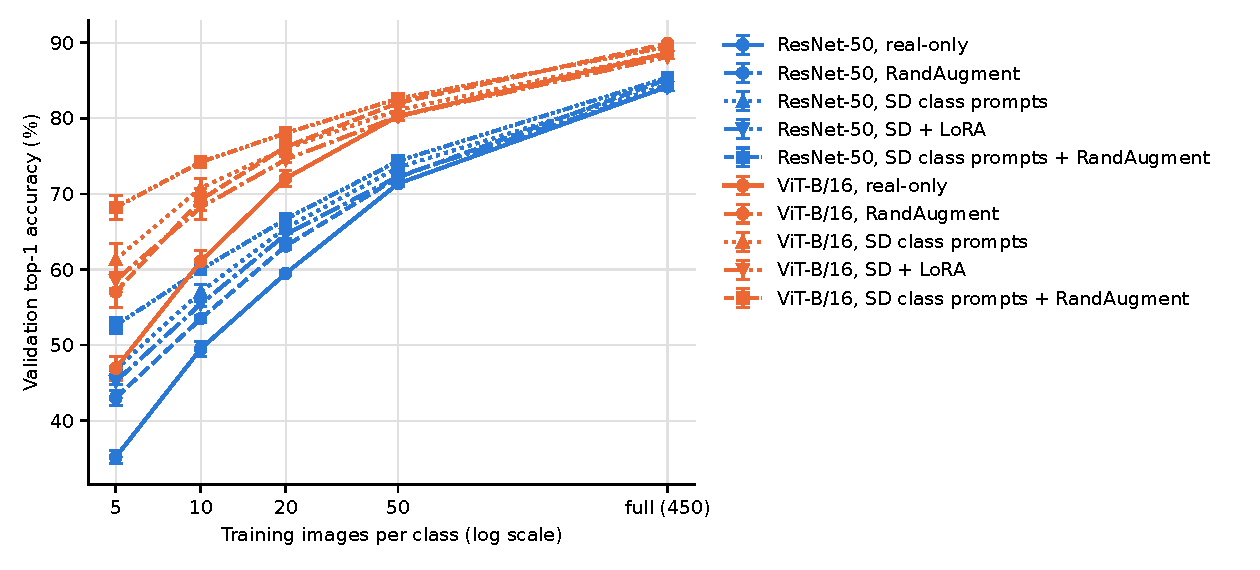
\includegraphics[width=\textwidth]{stage1_pretrained_all_conditions.pdf}
	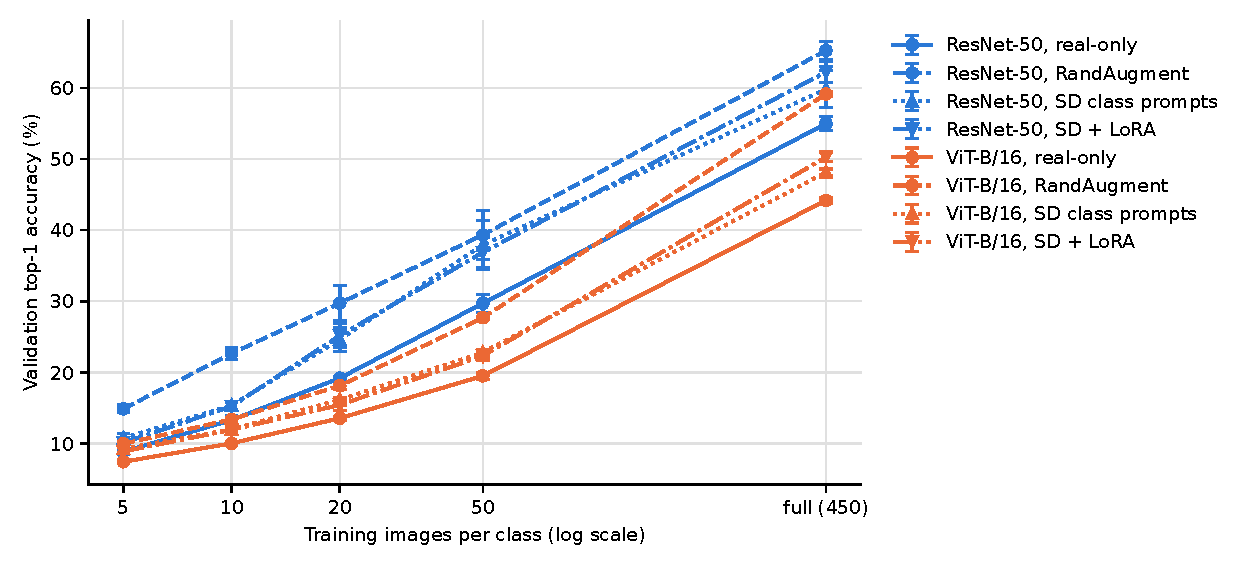
\includegraphics[width=\textwidth]{stage1_scratch_all_conditions.pdf}
	\caption{Validation top-1 accuracy of all Stage 1 conditions against training images per class (log scale), ImageNet-pretrained (top) and randomly initialized (bottom). Points are means over seeds 0, 1 and 2 with $\pm 1$ standard deviation; color marks the classifier, line style and marker the condition.}
	\label{fig:stage1-all-conditions}
\end{figure}
% Tables and figures generated by src/component/analyze_results.py --table/--figure from the run folders of both machines.

% ------------------------------------------------------------------------------------------------------------------------
\section{Discussion}

% Challenges, where the approach helps or fails, and what to try next.

% ------------------------------------------------------------------------------------------------------------------------
\section{Limitations}

% State the weaknesses before a reader finds them, and why they do not undermine the main claims:
% one dataset in Stage 1, 32x32 images upsampled to 224, three seeds, pretraining overlap
% (ImageNet, Stable Diffusion training data), single-GPU compute, stages not completed.

\textbf{One dataset at low resolution.} Stage 1 uses CIFAR-100 only, and its $32\times32$ images are upsampled to $224\times224$ for the classifiers. Results may differ for datasets with larger images or other domains, which later stages address.

\textbf{Three seeds.} With three training seeds, a gain or loss is declared only when all seeds agree, and the standard deviations are themselves uncertain. In the baselines, the standard deviation of the paired change reaches 4.7 points (ResNet-50 from random initialization, 50 images per class), so Stage 1 can resolve only effects larger than this spread; smaller effects will be reported as inconclusive. Stage 2 adds two more seeds.

\textbf{Fixed step budgets.} The step budgets were chosen in pilots on the real-only condition and are equal across conditions, so the comparison holds the training compute fixed. Some runs reached their best validation score at the final step: in the pretrained arm 1 of 30 real-only and 8 of 30 RandAugment runs, and in the random-initialization arm 6 of 30 and 13 of 30. Because the cosine schedule ends at a learning rate of zero, the last steps are often the best, but augmented runs might also gain from longer training, so the RandAugment gains may be understated. In the synthetic-data conditions the same step budget is spread over twice as many images, so each real image is seen about half as often as in the real-only run; the exposures are recorded for every run.

\textbf{Outside pretraining.} The ImageNet weights of the pretrained classifiers and the web-scale training data of Stable Diffusion are outside our control. The diffusion training data may contain images similar to, or taken from, CIFAR-100, so any benefit of generated images may partly reflect that exposure. The random-initialization arm removes the classifier's outside knowledge but not the generator's.

\textbf{Two software environments.} The synthetic-data runs were trained with newer Python, PyTorch, Torchvision and NumPy versions than the real-only and RandAugment runs they are paired with (Section~\ref{sec:protocol}). The recipe, split and step budgets are identical, but a version change can shift accuracy slightly, so small paired changes between the two groups should be read with that in mind; one baseline rerun in the newer environment will measure the size of this shift.

\textbf{Validation results so far.} The results reported here are validation scores. The test set will be scored once, after all Stage 1 conditions are trained.

% ------------------------------------------------------------------------------------------------------------------------
\section{Conclusion}

% Short answer to each research question.

% Lists every reference in references.bib while the text above is being written.
% Remove once all works are cited in the text.
\nocite{*}

\bibliographystyle{IEEEtran}
\bibliography{references}

\end{document}
